\documentclass[12pt,a4paper]{article}
\usepackage[latin1]{inputenc}
\usepackage{amsmath}
\usepackage{amsfonts}
\usepackage{amssymb}
\usepackage{graphicx}
\usepackage{dirtree}
\usepackage[left=1.00in, right=1.00in, top=1.00in, bottom=1.00in]{geometry}
\usepackage{hyperref}
\title{Monte Carlo Radiation Transfer (MCRaT)\\User's Guide}
\author{Tyler Parsotan}
\date{}
\usepackage{tabularx}
\usepackage{natbib}
\usepackage{subfig}
\usepackage{graphicx}
\bibliographystyle{apj.bst}
\begin{document}
\maketitle

\tableofcontents
\newpage

\section{Introduction}
The Monte Carlo Radiation Transfer (MCRaT; pronounced \textit{Em-Cee-Rat}) code is a next generation radiation transfer code that can be used to analyze the radiation signature expected from astrophysical outflows. The code is written in C and uses the Message Passing Interface (MPI) library for inter-process communication, the Open Multi-Processor (OpenMP) library for intra-node communication, the GNU Scientific Library, and the HDF5 library for parallel I/O.

MCRaT injects photons in a hydro simulation, using the FLASH or the PLUTO codes, and individually propagates and compton scatters the photons through the fluid until the end of the simulation. This process of injection and propagating occurs for a user specified number of times until there are no more photons to be injected. Users can then construct light curves and spectra with the MCRaT calculated results. The hydro simulation used in this version of MCRaT must be in 2D, however, the photon propagation and scattering is done in 3D by assuming cylindrical symmetry.

The code was initially written in python by Dr.\ Davide Lazzati as a proof of concept. The code was then translated into C by Tyler Parsotan and made to use the OpenMP, MPI, HDF5, and GNU Scientific libraries. MCRaT is highly parallelized and is easy to set up and use.


\section{Getting Started}
This section describes how to get the MCRaT code as well as the required libraries necessary to compile MCRaT. This section will also cover the necessary steps to run the compiled MCRaT code. 

\subsection{Required Libraries}
MCRaT requires a number of libraries in order to compile properly. These are:
\begin{itemize}
\item MPI
\item OpenMP
\item GNU Scientific Library (GSL)
\item HDF5
\end{itemize}

The MPI library can be an any implementation such as OpenMPI (\href{http://www.openmp.org/}{open-mpi.org}) or one that is specific to a given supercomputer. Following the steps to install the library should allow it to work properly for compiling MCRaT. The OpenMP library is automatically included with Intel and GNU compilers. The GNU Scientific Library (GSL) can be downloaded from \href{https://www.gnu.org/software/gsl/}{gnu.org/software/gsl/}. Following the included instructions should install GSL in the default directory for it to be found by the compiler. The HDF5 library can be found at \href{https://support.hdfgroup.org/HDF5/}{support.hdfgroup.org/HDF5/} where version 1.10 or greater should be downloaded and installed. The parallel portion of HDF5 needs to also be installed which is included in the instructions for installing HDF5.

\subsection{Downloading and Compiling MCRaT}
Once the required libraries have been installed, the current MCRaT code can be downloaded from \href{https://github.com/lazzati-astro/MCRaT/tree/master/HYBRID_PARALLEL_KN}{github.com/lazzati-astro/MCRaT/}. There is a Makefile which  makes compiling the code significantly easier. In the directory that all the MCRaT files were downloaded into, simply typing \texttt{make} will compile the MCRaT code into a binary file called \texttt{MCRAT}. Typing \texttt{make MERGE} will compile the included MCRaT post-processing code, which will be covered in later in this section, into a binary file called \texttt{MERGE}.

The Makefile has to be configured for a variety of specifics related to the user's system. The \texttt{CC} option in the makefile can be changed to the user's compiler of choice such as gcc or icc. The \texttt{HDF\_INSTALL} line is for the directory that the HDF5 library is installed in. The \texttt{EXTLIB} line is for the directories of any external libraries that the user may have. For example, if the GSL library cannot be found by the compiler, the user can put the directory of the library in this line of the Makefile in order to properly compile MCRaT. The \texttt{CFLAGS} feeds any compiler options to the compiler such as optimizations, and the switch to compile MCRaT with OpenMP capabilities, which is necessary to exploiting the hybrid parallelization available in the code. If the user is using gcc, the \texttt{-fopenmp} does not need to be changed, however, if the user is using icc, \texttt{-fopenmp} needs to be changed to \texttt{-qopenmp}. The \texttt{INCLUDE} line can be changed to include any \texttt{include/} directories to help the compiler, and the same if for the \texttt{LIBSHDF} in relation to any shared libraries. The \texttt{LIB}, \texttt{DEPS}, and \texttt{OBJ} lines should not need to be changed. Once the lines in the Makefile appropriately reflect the users configurations, typing \texttt{make} and \texttt{make MERGE} should properly compile the MCRaT code as well as its post-processing code, \texttt{MERGE}.

\subsection{The mcrat\_input.h file}
Once compilation is successful, the user will need to decide where MCRaT's output will go. The user needs to make a directory within the directory that contains the hydro simulation frames. This subdirectory is where the parameter file for MCRaT must be placed. This is the same directory in which MCRaT will do all of its work, including making its own directories and output files within the aforementioned directories. Once this directory is created, the user must modify the \texttt{mcrat\_inputs.h} file in order for the code to know where to find all the hydro files and the MCRaT parameter file. The constant \texttt{FILEPATH} should be modified with the directory of the flash simulation files while the constant \texttt{FILEROOT} should contain the name of the hydro simulation files without any frame numbers. The constant \texttt{MC\_PATH} should be the name of the directory, located within the \texttt{FILEPATH} directory, that holds the MCRaT parameter file named \texttt{mc.par}. An example file structure, with the values for each variable in MCRaT, is shown below: \\
\begin{figure}[h!]
\dirtree{%
.1 /dir/to/hydro/simulation/ (\texttt{FILEPATH}).
.2 dir\_with\_MCRaT\_parameter\_file/ (\texttt{MC\_PATH}).
.3 \texttt{mc.par}.
.2 example\_hydro\_file\_name\_0001 (\texttt{FILEROOT}=example\_hydro\_file\_name\_).
} 
\end{figure}

The other variable that can be changed in MCRaT is \texttt{SIMULATION\_TYPE} which should be set as \texttt{SCIENCE}, if using MCRaT for a production run, or \texttt{SPHERICAL}/\texttt{CYLINDRICAL} which is for testing MCRaT with these types of outflows (which will be covered in a later section). Once all the variables have been appropriately changed, by replacing the strings appropriately in the \texttt{mcrat.c} file, the code needs to be recompiled.

Additionally, there are a number of switches that the user can specify to the program to tell it whether they want to consider the effects of polarization, with the \texttt{STOKES\_SWITCH}, and one that specifies whether the user wants MCRaT to save the comoving 4 momenta of each photon, with the \texttt{COMV\_SWITCH}. These switches can be set to \texttt{OFF}, which means do not save the comoving 4 momenta and/or save and consider the effects of polarization, or they can be set to \texttt{ON}, which tells the program to consider polarization and/or save the stokes parameter associated with each photon or save each photon's 4 momentum.

The \texttt{SIM\_SWITCH} tells MCRaT what hydro simulation is being used. The options are \texttt{FLASH} and \texttt{PLUTO\_CHOMBO}, for the FLASH hydrodynamic code and the PLUTO hydro code with CHOMBO AMR. The switch \texttt{DIM\_SWITCH} tells MCRaT the dimensionality of the hydro simulation that is used. This switch can be set to \texttt{2}, for 2D, or \texttt{3}, for 3D. The 3D feature is still in development so the switch should be set to \texttt{2} for now. The geometry can also be specified through the \texttt{GEOMETRY} define statement. The options are \texttt{SPHERICAL} and \texttt{CARTESIAN}; however, since MCRaT only supports 2D, the supported spherical coordinate system is $(r, \theta)$ and the supported \texttt{CARTESIAN} system is $(x,y)$ and $(r,z)$ in cylindrical coordinates. The length scale of the hydro simulation also has to be specified by setting the value of \texttt{HYDRO\_L\_SCALE} to the normalization that is used in the hydro simulation.

The parameters that can be set and the appropriate values that each parameter can be set as are as follows:
\begin{figure}[h!]
\centering
%\begin{table}
\begin{tabular}{|c|p{0.5\textwidth}|}
\hline 
Parameter & Acceptable Values \\ 
\hline 
SIMULATION\_TYPE & SCIENCE,\newline CYLINDRICAL\_OUTFLOW, \newline SPHERICAL\_OUTFLOW, \newline STRUCTURED\_SPHERICAL\_OUTFLOW \\ 
\hline 
FILEPATH & ``/dir/to/hydro/simulation/ '' \\ 
\hline 
FILEROOT & ``example\_hydro\_file\_name '' \\ 
\hline 
MC\_PATH & ``dir\_with\_MCRaT\_parameter\_file/'' \\ 
\hline 
SIM\_SWITCH & FLASH, PLUTO\_CHOMBO \\ 
\hline 
STOKES\_SWITCH & ON, OFF \\ 
\hline 
COMV\_SWITCH & ON, OFF \\ 
\hline 
DIMENSIONS & 2 \\ 
\hline 
GEOMETRY & CARTESIAN, SPHERICAL \\ 
\hline 
HYDRO\_L\_SCALE & $(-\infty, +\infty)$ \\  
\hline 
MCPAR & ``mcpar\_filename.par'' \\ 
\hline 
\end{tabular} 
%\end{table}

\end{figure}

\subsection{The MCRaT Parameter File} \label{mc.par}
MCRaT requires the user to provide information in the form of a parameter file named \texttt{mc.par} which should be placed in the appropriate directory, as is described in the previous section. An example \texttt{mc.par} file, named \texttt{sample\_mc.par} is included in the MCRaT github repository. An example with a description of each line, is as follows:\\

\begin{tabularx}{\linewidth}{r X}
1e12 &   The 1$^\textrm{st}$ line is the domain of the hydro x axis \\ 
1e13 &   The 2$^\textrm{nd}$ line is the domain of the hydro y axis \\ 
5 &   The 3$^\textrm{rd}$ line is the the hydro simulation number of frames per second  \\ 
200 &    The 4$^\textrm{th}$ line is the starting frame number for angles $\le 2^\circ$\\ 
200 &   The 5$^\textrm{th}$ line is the starting frame number for angles $> 2^\circ$ \\ 
3000 &   The 6$^\textrm{th}$ line is the last hydro frame number \\ 
124 &    The 7$^\textrm{th}$ line is the number of frames in which photons are injected for angles $\le 2^\circ$\\ 
124 &   The 8$^\textrm{th}$ line is the number of frames in which photons are injected for angles $> 2^\circ$ \\ 
8e11 &    The 9$^\textrm{th}$ line is the radius at which the photons will be injected for angles $\le 2^\circ$\\ 
9e11 &   The 10$^\textrm{th}$ line is the radius at which the photons will be injected for angles $> 2^\circ$ \\ 
0 &   The 11$^\textrm{th}$ line is the minimum angle in degrees for which photons will be injected \\ 
20 &   The 12$^\textrm{th}$ line is the maximum angle in degrees for which photons will be injected \\ 
4 &   The 13$^\textrm{th}$ line is the change in angular resolution, this partly dictates how MCRaT will parallelize the simulation \\ 
5e50 &   The 14$^\textrm{th}$ line is the users initial guess of the weight of each injected photon for angles $\le 2^\circ$ \\ 
5e50 &    The 15$^\textrm{th}$ line is the users initial guess of the weight of each injected photon for angles $> 2^\circ$\\ 
1000 &   The 16$^\textrm{th}$ line is the minimum number of photons the user wants injected in each frame \\ 
3000 &    The 17$^\textrm{th}$ line is the maximum number of photons the user wants injected in each frame\\ 
b &   The 18$^\textrm{th}$ line is the spectrum of the injected photons. ``b''=Blackbody and ``w''=Wein \\ 
r &    The 19$^\textrm{th}$ line is to tell MCRaT to start a new simulation, ``r'', or continue an old one, ``c'' \\ \newline
\end{tabularx} 

There are values related to photons injected within $2^\circ$ and outside of $2^\circ$ because at this angle, the outflow may become significantly denser (as occurs in Gamma Ray Bursts) and the user may want to increase their radius of injection in order to speed up the computation. In order to match the time in which photon injection will occur at these larger angles means changing the parameters that play a role in the value of the simulation time when the photons begin being injected. 

Lines 4 combined with line 9 dictate what time in the simulation you begin injecting photons. This is calculated as 
\[
t_\mathrm{start}=\frac{\mathrm{f_{start}}}{\mathrm{fps}}-\frac{R_\mathrm{inj}}{c}
\]
where $\mathrm{f_{start}}$ is the value in line 4, fps is the frames per second which is the value in line 3, $R_\mathrm{inj}$ is the radius at which photons are injected, or the value in line 9, and c is the speed of light. Building on the above formula, the time in which photons stop being injected are calculated as
\[
t_\mathrm{end}=\frac{\mathrm{f_{start}}+\mathrm{df}}{\mathrm{fps}}-\frac{R_\mathrm{inj}}{c}
\]
where df is the number of frames in which photons are injected, which is line 7. These calculations are the same for photons injected at angles $> 2^\circ$, except you use the \texttt{mc.par} lines that are applicable to those photons in the calculations. 

Line 19 allows the user to continue the MCRaT code from a previous point, if the value is set to ``c'', or it allows the user to restart (by erasing the full working directory of MCRaT) or start a simulation by setting it to ``r''. {\bf This is an important parameter to check to prevent accidentally erasing work that has already been done.}

Line 13 should be a value that divides evenly into the angle range provided by lines 12 and 11. In the above example (20-0)/4=5. This is important for MCRaT's parallelism. Another number that MCRaT uses to break up the problem is lines 7 and 8. The way that MCRaT parallelizes the problem will be shown in the next section.

\subsection{Understanding MCRaT's Parallelism}
The first step that MCRaT takes in breaking up the problem is breaking it up into pieces based on the range of angles that photons will be injected into, which the user specifies in lines 11 - 13 in the \texttt{mc.par} file. As the example \texttt{mc.par} above shows, MCRaT will break up the problem into (20-0)/4=5 pieces initially. Then, for each angle range ($0^\circ-4^\circ$, $4^\circ-8^\circ$, etc.) the code will then break up the problem based upon how many times photons will be injected, which is 1 plus the values in lines 7 and 8 in the \texttt{mc.par} file; this is because the photons are injected in the frames $[\mathrm{f_{start}}, \mathrm{f_{start}}+1, ..., \mathrm{f_{start}}+\mathrm{df}-1, \mathrm{f_{start}}+\mathrm{df}]$, which gives us this n+1 behavior. These pieces of information are important for understanding how the processes are divided with MCRaT. An example will be given in the next section.

\subsection{Running MCRaT}
In this section we show how to run MCRaT and allocate the appropriate number of cores in order to optimize MCRaT's parallelism. We will use the example \texttt{mc.par} file in Section \ref{mc.par} for this section. 

Running the MCRaT code is as simple as doing \texttt{mpiexec -np N ./MCRAT} where N is the total number of MPI processes that will be created. The OpenMP parallelism is controlled by setting the OpenMP environment variable \texttt{OMP\_NUM\_THREADS}. We recommended that \texttt{OMP\_NUM\_THREADS} be set to $1$ for a newly started MCRaT simulation, which essentially turns off the OpenMP parallelism. 

 The total number of MPI processes, N, is initially divided by the set of angles that photons will be injected into. For the example \texttt{mc.par}, there are $(20-0)/4=5$ sets of angles that will be considered which leads to the N MPI process initially being divided by 5. The $N_\theta=N/5$ MPI processes will then be used to inject photons in the user specified frames in parallel. The example \texttt{mc.par} file shows that there will be 124+1 photon injections, as was described in the last section. Thus, the number of frames that each MPI process will inject photons into becomes $\mathrm{f_{inj}}=(124+1)/N_\theta$. If we set $N=125$, $N_\theta=25$ and the number of frames that each MPI process will inject photons into becomes 5. Alternatively, if we want each MPI process to only inject photons into one frame, $N_\theta=125$ which means that $N=625$. Calculating N by following these examples, shows how the problem is broken up between angles and photons injections. If the number of MPI processes available for the user to use does not divide well into the size of the problem, in terms of angle ranges and frames in which photons are injected, MCRaT will prioritize breaking up the problem evenly based on the set of angles. Thus, $N$ should at least be evenly divisible by the number of angle ranges specified by the \texttt{mc.par}; Once $N_\theta$ is calculated, MCRaT will distribute the number of frames in which photons will be injected accordingly to calculate $\mathrm{f_{inj}}$.
 
 Another option, when dealing with a limited number of available cores, is running MCRaT on a small portion of the problem. For example instead of doing 5 sets of angles at $4^\circ$ intervals all at once, simply run 1 set of angles from $0^\circ-4^\circ$, and when that simulation is complete run the second set from $4^\circ-8^\circ$, etc. The increased parallelism in decreasing $\mathrm{f_{inj}}$ by using this method may speed up the simulation compared to running the whole problem at once. This is also advantageous due to the fact that as the MPI processes begin to complete their portion of the simulation, the user may restart MCRaT using only the appropriate number of MPI processes left that have calculations left to do. Thus, this feature lets a given MCRaT simulation (e.g. $0^\circ-4^\circ$) use less MPI processes and resources over time, allowing another full simulation (e.g. $4^\circ-8^\circ$) to start running using the rest of the available resources. We will go over this feature in a later section.
 
 \subsection{MCRaT Output}
 Once MCRaT is run, it will create subdirectories dedicated to the calculations and results of each angle range. Using the example \texttt{mc.par} file, the directory tree will now look like: 
 
 \begin{figure}[h!]
 \dirtree{%
 .1 /dir/to/hydro/simulation/.
  .2 example\_hydro\_file\_name\_0001.
 .2 dir\_with\_MCRaT\_parameter\_file/.
 .3 \texttt{mc.par}.
 .3 0.0-4.0/.
 .4 mc\_proc\_$i$.h5.
 .4 mc\_chkpt\_$i$.dat.
 .4 mc\_output\_$i$.log.
 .3 4.0-8.0/.
 .4 mc\_proc\_$i$.h5.
  .4 mc\_chkpt\_$i$.dat.
  .4 mc\_output\_$i$.log.
 .3 8.0-12.0/.
 .4 mc\_proc\_$i$.h5.
  .4 mc\_chkpt\_$i$.dat.
  .4 mc\_output\_$i$.log.
 } 
 \end{figure}
 
 We have not included the subdirectories extending up to $20^\circ$ for brevity, but those other 2 directories would also be created. Within each angle subdirectory, each MPI process, labeled process $i$, creates 3 files. The mc\_output\_$i$.log file prints exactly what the MCRaT code is doing for that given MPI process. This allows us to monitor the progress of the MCRaT simulation. This can be easily done by using Linux commands such as \texttt{less mc\_output\_$i$.log}. The mc\_proc\_$i$.h5 is a HDF5 file that contains all of the calculation results of the MCRaT MPI process. The mc\_chkpt\_$i$.dat file contains the necessary data for each MPI process to continue from the last point if MCRaT is interrupted for any reason. This is covered in the next section.
 
 When all of the MPI processes in a given angle subdirectory have completed their calculations, they will produce HDF5 files with the results of the calculations for each file in the simulation starting with the frame specified in line 4 (or 5, depending on the angle range under consideration) in the \texttt{mc.par} file up to the frame specified in line 6 in the \texttt{mc.par} file. These files will be named \texttt{mcdata\_$f$.h5} where $f$ is the frame number of the hydrodynamic simulation.
 
 \subsection{Restarting MCRaT}
 If the MCRaT code gets interrupted by running out of allocated time on a cluster or any other type of issue, the code is easily continued and it may also use less MPI processes when it is restart based on the number of MPI processes in the original simulation run that still have calculations to complete. 
 
 In order to ensure that the code knows to continue a MCRaT simulation, the 19$^\textrm{th}$ line in the \texttt{mc.par} file must be set to ``c''. {\bf This is important to check since not changing this parameter means that all of the simulation progress will be erased and a completely new simulation will be started, thus nullifying the attempt to save time and resources by continuing a MCRaT simulation.} 
 
 Once this parameter has been changed, the user needs to identify how many total MPI processes have completed their calculations. This is done by running \texttt{tail -n 1 dir\_with\_MCRaT\_parameter\_file/angle\_dir/mc\_output\_* |grep "completed" |wc -l} in each angle range directory created by MCRaT. Add all the printed values and subtract from the original number of MPI processes, $N$, that the MCRaT simulation was started with. This is the number that has to replace $N$ in the new run of MCRaT. From here, MCRaT automatically distributes the given number of processes among the MPI processes in each angle subdirectory that still need to run calculations.
 
 This feature of only continuing the MCRaT simulation with the necessary number of MPI processes means that as the simulation progresses, fewer resources will be used which is invaluable for running jobs in a pipeline type of fashion and for conserving resources such as SBU allocations.
 
 If a certain process is also taking a long time to conduct its simulation it is possible to modify the mc.par file to specify that the simulation should inject fewer photons, to speed up the calculation and force the process's simulation portion to restart. To force the restart delete that processes mc\_chkpt file and it's  mc\_proc file. This is exactly what the \texttt{mcrat\_msp.sh} shell script does. 
 
 \subsubsection{Using The mcrat\_msp.sh Shell Script}
 The mcrat\_msp.sh shell script determines which MCRaT processes have a very large number of scatterings and allows the user to delete those process' mc\_chkpt and mc\_proc files, if the process' photons have undergone a number of scatterings greater than some user specified number of scatterings, which would then force a new restart for those processes with less injected photons. It also allows the user to refine the mc.par file to set a new number of injected photons for these same processes that will be restarted the next time the user starts mcrat with the 'c' flag to continue a simulation. {\bf This is important to change once MCRaT has been restarted and the photons injected. If it isn't other processes, which don't have so many scatterings, will inject photons (if applicable, which it should be on a relatively small cluster where the user can't assign one photon injection frame to each process) within the new range specified by the mc.par file. To do this, once the simulation restarts and is running smoothly, the user has to end it, modify the minimum and maximum range of injected photons to the original numbers, and restart the simulation once again. (We are currently working on a better way of implementing this feature.) The user must remember to reset the restart flag in the mc.par file to 'c' otherwise all the simulation data files will be erased and all progress lost.} Opening the mcrat\_msp.sh file in a text editor will bring up different flags for the shell script and give examples of how to properly use the function.
 
 \subsection{Using Hybrid-Parellelization}
 As was mentioned earlier, it is not advised to enable hybrid parallelization at the start of a new MCRaT simulation, especially if limited resource availability is an issue. This is due to the fact that the OpenMP threads may interfere with one another and neighboring MPI processes and their OpenMP threads, thus slowing the overall code. To prevent this, set \texttt{OMP\_NUM\_THREADS} to $1$.
 
 If MCRaT is being used to continue a simulation, there is a good chance that some of the MPI processes have finished and the remaining MPI processes are running slower than the rest due to a variety of factors, which will be covered later. Thsi is where hybrid parallelization helps to ensure that MCRaT completes its calculations is a reasonable amount of time. These MPI processes can be sped up by using the OpenMP threads. The number of threads per MPI process can be set with the \texttt{OMP\_NUM\_THREADS} parameter. Even in this case, it is important to make sure that threads are not interfering with one another and undermining any potential performance gain.
 
 \subsection{Post-Processing MCRaT Data}
 If the user is simply running running a simulation with one angle range under consideration, there is no post-pocessing to be done. The MCRaT produced \texttt{mcdata\_$f$.h5} files contain all the information for the photons (which will be covered in the next section).
 
 If not we need to be able to merge all the simulation results for photons injected in all angle ranges; following the example \texttt{mc.par} file, we need to merge the data in angles $0^\circ-4^\circ$, $4^\circ-8^\circ$, etc. This is done is with the MERGE code that is included with MCRaT. To run merge, the user simply types \texttt{mpiexec -np N ./MERGE}. In this case N needs to be a multiple of the number of subdirectories the MCRaT code has created and it has to be greater than or equal to the number of subdirectories; of cource the larger the number of MPI processes used, the less work each process has to do, making the post-processing code faster. In the example \texttt{mc.par} file there are 5 directories created, so N has to be a multiple of 5 in this case. The minimum value of N can be 5; however, since the MERGE code is also parallelized with OpenMPI, the larger the number of processes used, the less time it takes to merge all of the MCRaT data.  If $N=10$, 5 processes will be allocated to merge the data from the first half of the frames from 200 to 3000, as specified in the \texttt{mc.par} file, and the other 5 will merge the data from the last half of the range of frames.
 
 The merged data is placed into another folder that the code creates named \texttt{ALL\_DATA/}. \newline
 
 \noindent The standard work flow for MCRaT is as follows:
 \begin{itemize}
 \item[1.] Compile the MCRaT and MERGE codes
 \item[2.] Write the \texttt{mc.par} file in the correct directory
 \item[3.] Run MCRaT
 \item[4.] use MERGE to post-process the MCRaT results
 \end{itemize}
 
 This work flow can be practiced using a spherical or cylindrical outflow problem that is included in MCRaT. These simulations can be run using any hydro simulation because MCRaT reads in the data from the hydro simulation and over writes it (in memory, not in the hydro file) with the correct values assuming a spherical or cylindrical outflow.
 
 In order to run a spherical outflow simulation simply change the \texttt{SIMULATION\_TYPE} parameter in \texttt{mcrat\_inputs.h} file to \texttt{SPHERICAL}. Then recompile the code and run it as we outlined previously. In order to run a cylindrical outflow simulation, change the \texttt{SIMULATION\_TYPE} parameter to \texttt{CYLINDRICAL}. These test simulations allow the user to become acquainted with MCRaT and test that MCRaT produces the expected results for these type of outflows.
 

\section{The MCRaT Code}
This section describes the algorithm and output of MCRaT. It will cover the steps that MCRaT takes to inject and scatter photons.

\subsection{Assumptions about the RHD Simulation}
MCRaT has to make some assumptions about the output of the RHD simulation. These assumptions are:
\begin{itemize}
\item[1.] The velocity in the RHD simulation is normalized by the speed of light, $c$ 
\item[2.] The pressure is normalized by $c^2$
\item[3.] The density is normalized by $1$
\end{itemize}

\subsection{Algorithm}\label{algorithm}

MCRaT first reads the data from the \texttt{mc.par} file and then appropriately divides the MPI processes based on the number of angle ranges, if starting a new simulation, or, for continuing a simulation, reads the mc\_chkpt file in each directory to determine which MPI processes still have work to complete and then distributes the MPI processes. 

Each MPI process is assigned a range of frames in which the process injects photons into and then propagates through all the hydro simulation frames until the last hydro simulation frame, which is specified in the \texttt{mc.par} file. The photons have a \texttt{photon} data structure that fully describes each photon. This includes the photon's lab frame 4-momenta, the x, y, and z coordinates of the photon, the Stokes parameters of the photon, the weight of the photon, the number of times the photon has scattered, and the index of the hydro fluid element that the photon is located within.

In order to inject the photons, MCRaT reads in the first hydro frame in which the photons will be injected in and chooses hydro elements that have radii, $r$, such that $R_\mathrm{inj}-c/(2*\mathrm{fps}) < r < R_\mathrm{inj}+c/(2*\mathrm{fps})$, where $c$ is the speed of light, $R_\mathrm{inj}$ is the injection radius and $\mathrm{fps}$ is the hydro simulation frames per second, both specified in \texttt{mc.par}. These hydro elements also have to be within the angle range that the MPI process is injecting photons within. Thus, we choose a slab of hydro elements to inject photons into. The number of photons that would be expected from the $i^\mathrm{th}$ hydro element, $n_i$, is calculated using the energy density of the element and by assuming a weight for each MCRaT photon which is taken from the \texttt{mc.par} file. This is further explained in Section \ref{inj}. Once the expected number of photons is calculated, the actual number is acquired by assuming that the photon injection is random, which means that we acquire the actual number of photons injected into the $i^\mathrm{th}$ hydro element, $N_i$ by randomly drawing from a Poisson distribution with a mean of $n_i$. The total number of photons that would be injected across all the chosen hydro elements becomes $N=\sum N_i$. If $N$ is within the minimum and maximum number of photons that the user wants, which is specified in the \texttt{mc.par} file, the calculation for the number of photons is complete. If not, then the code continues to recalculates $n_i$ using a new weight for each photon, then recalculates $N_i$ and $N$, and after rechecks so see if $N$ is within the user specified number of photons again. This loop is exited when $N$ falls within the user specified number of desired photons. If the code needs to inject more photons to meet this condition, it will adjust the weights to be smaller and vice versa.

Once $N$ and $N_i$ have been determined, the $N_i$ photons are placed at the center of the $i^\mathrm{th}$ hydro element, with a random azimuthal angle uniformly distributed between $0$ and $2\pi$ (since we assume cylindrical symmetry for the 2D hydro simulation), and they are given an energy based on the comoving temperature of the hydro element, thus the photons are injected in the comoving frame fo the outflow. If the user specified that the photons should be injected with a Wien spectrum then the frequencies, $\nu$, are assigned to the $N_i$ photons by sampling from a Wien spectrum defined by the $i^\mathrm{th}$ fluid element's comoving temperature. The same thing is done with a Blackbody spectrum if the user specified that the photons should be injected as a Blackbody spectrum. This sampling is done by using the acceptance-rejection Monte Carlo sampling of the spectra.

For their 4-momenta, the photons are assigned a random azimuthal angle, $\phi$, from a uniform distribution between $0$ and $2\pi$, as well as a polar angle, which is calculated as $\theta=\arccos(2\xi-1)$, where $\xi$ is a random number drawn from a uniform distribution. The $i^\mathrm{th}$ injected photon 4-momentum becomes:
\[
p^\mu_i=\frac{h\nu_i}{c}\begin{pmatrix}
1 \\ \sin(\theta_i) \cos(\phi_i) \\ \sin(\theta_i) \sin(\phi_i) \\ \cos(\theta_i)
\end{pmatrix}
\]

After the 4-momenta are set, the photons are boosted into the lab (observer) frame using the velocity of the fluid element that the photons are located within. The lab frame 4-momenta are saves to each photon's \texttt{photon} data structure, as well as the photon's position and weight. The number if scatterings is initialized to 0 and the stokes parameters are initialized to 0 except for s0 which is set to 1.

Once the photons have been injected into the simulation and their 4-momenta have been determined, the scattering process through the hydrodynamic (HD) simulation occurs. MCRaT reads in a HD simulation frame, starting from the frame in which the photons were initially injected into up until the last HD simulation frame available, and determines which HD fluid elements each photon is in and then calculates the mean free path of each photon. In order to reduce memory and optimize the code, MCRaT determines the minimum and maximum radii of the photons, $R_\mathrm{min}$ and $R_\mathrm{max}$ respectively, and selects a slab of hydro fluid elements with radii, $r_i$ such that 
\[
R_\mathrm{min}-\alpha\frac{c}{\mathrm{fps}} < r_i < R_\mathrm{max}+\alpha\frac{c}{\mathrm{fps}} 
\] 
where $\alpha$ is a multiplicative factor that can be increased to ensure that the number of chosen hydro elements is greater than 0. The code finds which fluid element each photon is located within, and saves the index to the \texttt{photon} data structure. This data field only gets updated if the photon propagates outside of the fluid element. If this happens, then the code finds and saves the index of the new fluid element that the photon is located within. Sometimes, the code is not able to find a fluid block that a given photon is located within. This may happen due to a photon propagating outside of the range of radii of the chosen slab of hydro element, and is very rare. To deal with this, we set the mean free path, $l$, to an arbitrary large value to ensure that the photon doesn't scatter, which would inaccurately change its energy. If the fluid element is correctly identified, the mean free path is calculated as  
\[
l=-\frac{m_p}{\rho\sigma_\mathrm{T}(1-\beta\cos\theta_{fp})}\ln\xi
\]
where we have inverted the exponential probability distribution for a photon scattering in a medium. Here, $\xi$ is a random number uniformly distributed between 0 and 1, $m_p$ is the proton mass, $\sigma_\mathrm{T}$ is the Thompson cross section, $\rho$ is the lab frame density of the hydro fluid element that the photon is located within, $\beta$ is the velocity of the fluid element normalized by the speed of light (this should be already done in the hydro code), and $\theta_{fp}$ is the angle between the fluid element's and the photon's velocity vectors. From $l$, the time for each photon to scatter is calculates as $t_\mathrm{s}=l/c$, where $c$ is the speed of light. The photon with the smallest $t_s$ is assumed to scatter first, however that is not necessarily true since we use the full Klein-Nishina cross section in the electron rest frame to actually determine if the scattering occurs. The positions of all the photons are advanced by the time for the photon of interest to scatter, $t_s$.

In determining whether a photon will scatter or not, we first boost the chosen photon with the smallest $t_s$ to the fluid rest frame and produce an electron by sampling the Maxwell-Boltzmann or Maxwell-Juttner distributions for non-relativistic and relativistic gases. The comoving temperature, $T_i'$, of the fluid element is used to distinguish between which distribution is used. If $T_i' \ge 1 \times 10^7$ K the Maxwell-Juttner distribution is used, otherwise the Maxwell-Boltzmann distribution is used. When the Maxwell-Boltzmann distribution is used we choose 3 random x, y and z velocities from gaussian distributions with a standard deviation of $k_BT_i'/m_e$, where $k_B$ is the Boltzmann constant and $m_e$ is the mass of the electron. The velocities are normalized by the speed of light and used to calculate the Lorentz factor of the electron in the fluid frame. To get the full 4-mometum of the electron, the azimuthal angle of the electron's direction fo travel is drawn from a uniform distribution between 0 and $2\pi$ and the polar angle is acquired by acceptance-rejection sampling of the polar angle distribution $(1-\beta\cos(\theta))\sin(\theta) $. We then perform rotations based on the velocity vector of the photon that will scatter to ensure that the electron velocity is oriented relative to the photon's velocity.

Once the electron has been initialized, the photon and the electron are boosted into the electron rest frame. Then the photon velocity vector is rotated such that it is directly along the x-axis with the stationary electron at the origin of the coordinate system. We then use the Klein Nishina (KN) cross section including the effects of polarization, $\sigma_\mathrm{KN}$, to determine if the photon will actually scatter. The ratio $\sigma_\mathrm{KN}/\sigma_T$ is calculated and a random number, $\xi$, from a uniform distribution between 0 and 1 is drawn. If $\xi >\sigma_\mathrm{KN}/\sigma_T $ the photon does not scatter, otherwise it does scatter with the electron. 

If the photons scatters with the electron, a random $\theta$ and $\phi$ are drawn from their respective distributions that are derived from the KN cross section including polarization. The photon's new 4-momentum and stokes parameters are calculated and then the scattered photon is rotated to its original orientation with respect to the previously stationary electron. The photon is then Lorentz boosted twice, back to the lab frame. The process of keeping track of the Stokes parameters and calculating them will be covered in \autoref{pol}.

If the photon does not scatter, then the next photon with the second shortest time to scatter is chosen and the process to create an electron and determine if the photon will scatter repeats. This loop continues until a photon scatters or all of the photons have been determined to not scatter. 

While this loop is occurring, the photons in the simulation are being propagated incrementally by the change in scattering time for each photon until the time for the next hydro simulation frame is reached. The same thing occurs when a photon does scatter, the photons get propagated through space using the scattering time and the process of determining each photons' time to scatter, etc. repeats until the time corresponding to the next hydro frame is reached.

Once the time limit for the next hydro fluid frame is reached, MCRaT saves all the photons' information in the \texttt{photon} data structure into the HDF5 file under a group with the same hydro fluid frame number that the photons were being scattered in. Once the data is written, a checkpoint file is saved for MCRaT to be able to continue the simulation if it were interrupted. Then, the next simulation frame is loaded and the process of determining photons' time to scatter, actual probability of scattering and resulting scattered 4-momenta until the next HD simulation frame time is reached. This repeats until the last HD simulation frame is reached. 

If the MPI process has more photons to inject, then the process of injecting the photons into the next frame and propagating those photons through the hydro simulation repeats. If all of the MPI processes have finished injecting and propagating photons for the hydro simulation frames assigned to them, the code combines all of the photons' data from each MPI process into \texttt{mcdata\_$i$.h5} files where $i$ is the hydro simulation frame number. The output is covered in the next section.

\subsection{Output} 

Each MCRaT MPI process outputs 3 files. These files are named \texttt{mc\_proc\_$i$.h5}, \texttt{mc\_chkpt\_$i$.dat}, and \texttt{mc\_output\_$i$.log} where $i$ is the number for the MPI process producing those files. As the end of the simulation, MCRaT produces the actual data files named \texttt{mcdata\_$f$.h5} where $f$ is the hydro simulation file frame.

The \texttt{mc\_chkpt\_$i$.dat} file is a binary file that contains the data from the MPI process that allows it to continue the simulation if MCRaT gets interrupted for any reason. This information is: the MPI process' range of hydro frames to inject photons into, the frame that the current set of photons were injected in, the frame in which the photons were recently scattered in, the current time of the MCRaT simulation, the number of photons that the code is keeping track of, and the \texttt{photon} data structure for each photon in the simulation.

The \texttt{mc\_proc\_$i$.h5} file is a HDF5 file that contains all the data for the photons that the $i^\mathrm{th}$ MPI process injects and propagates through the hydro simulation. The data is organized by the hydro simulation frame which constitutes a HDF5 group. Within the group, there are the following datasets, depending on if \texttt{STOKES\_SWITCH} or \texttt{COMV\_SWITCH} id set to ON or OFF.
\begin{itemize}
\item PW - The photon weight for any photons that were injected into the frame. If there were no photons injected, then this data set does not exist.
\item P0 - the energy of the photons
\item P1 - the magnitude of the photons' 4-momentum in the x direction
\item P2 - the magnitude of the photons' 4-momentum in the y direction 
\item P3 - the magnitude of the photons' 4-momentum in the z direction
\item COMV\_P0 - the comoving energy of the photons
\item COMV\_P1 - the magnitude of the photons' comoving 4-momentum in the x direction
\item COMV\_P2 - the magnitude of the photons' comoving 4-momentum in the y direction 
\item COMV\_P3 - the magnitude of the photons' comoving 4-momentum in the z direction
\item R0 - the x position of the photons
\item R1 - the y position of the photons
\item R2 - the z position of the photons
\item S0 - the I Stokes parameter for the photons
\item S1 - the Q Stokes parameter for the photons
\item S2 - the U Stokes parameter for the photons
\item S3 - the V Stokes parameter for the photons
\item NS - the cumulative number of scattering each photon has undergone
\end{itemize}

These data sets include information for all of the photons after they were scattered through the given hydro simulation frame. The order of the data is based on the chronological order in which each set of photons were injected. For the example \texttt{mc.par} file in \autoref{mc.par}, if the user uses $N$ MPI processes such that each process injects photons into 2 frames, the \texttt{mc\_proc\_$0$.h5} file would look like:
\begin{figure}[h!]
 \dirtree{%
 .1 \texttt{mc\_proc\_0.h5}.
  .2 200.
  .3 PW.
  .3 P0.
  .3 $\colon$.
  .3 NS.
 .2 201.
   .3 PW.
   .3 P0.
   .3 $\colon$.
   .3 NS.
 .2 202. 
 	.3 P0.
    .3 $\colon$.
    .3 NS.
 } 
 \end{figure}
 
\newpage where all the datasets in group 200 would have only $n_{0}$ elements, where $n_{0}$ is the number of photons first injected into hydro frame 200. If we let $n_{1}$ be the number of photons injected in frame 201, the dataset PW in group 201 will have $n_{1}$ elements while the rest of the datasets will have $n_{0}$ elements, corresponding to the information for the photons first injected in frame 200 that are propagated through frame 201, \textit{followed by} $n_{1}$ elements for the newly injected photons in frame 201. 

The last file produced by the MCRaT MPI processes are named \texttt{mc\_output\_$i$.log}. These are files that output the progress of the given process, allowing the user to keep track of how far along MCRaT is in the radiation transfer simulation and how much more work the code has left to complete. This file contains the number of scatterings that the code completes in increments of 1000 scatterings as well as the average photon energy in units of ergs, the comoving temperature, in Kelvin, of the hydro fluid element that was used in the most recent scattering, and the most recent time step for a photon to scatter and the current time in the simulation. When all the scatterings are completed for a given frame, the code prints out the average cumulative number of scatterings that each photon has undergone, as well as the the maximum and minimum number of scatterings for the photons.The code also prints out the average radius of the MCRaT photons, the simulation time and the frames left to inject photons into and the last hydro simulation frame.

When the MCRaT MPI process has completed the Monte Carlo scattering portion of the code it will print: ``Process $i$ has completed the MC calculation.'' where $i$ is the ID of the MPI process. When all of the MPI processes are complete with the Monte Carlo scattering they will collectively produce the \texttt{mcdata\_$f$.h5} files which contain the merged data from each MPI process within a given angle range.

These \texttt{mcdata\_$f$.h5} files are formatted in the same way that the HDF5 groups are formatted in the \texttt{mc\_proc\_$i$.h5} files. The only exception is that there is a \texttt{PW} dataset with the weight of the photons being in the chronological order of photon injection.

\subsection{Post-processing Algorithm}
When the user has completed running MCRaT for each angle range that they are interested in, the data for every simulated photon gets merged into a new directory called \texttt{ALL\_DATA}. the MERGE code that is included with the download of MCRaT uses parallel HDF5 I/O to speed up this post-processing. 

The code takes the MPI processes and distributes them evenly among the MCRaT produced angle subdirectories. If there are $n_\theta$ angle subdirectories, the MPI processes are grouped into sets of $n_\theta$, with each MPI process operating withing a given subdirectory. Then, the code distributes the hydro simulation frames that need to be created among the groups of $n_\theta$ MPI processes. It also counts how many processes were originally used by MCRaT in each directory so if MCRaT is independently run 3 different times for 3 different ranges of angles, but with each of the 3 runs using a different number of MPI processes, the post-processing code will still work.

These processes open the \texttt{mc\_proc\_$i$.h5} files and tally how many photons will be merged to produce the final \texttt{mcdata\_$f$.h5} file in the \texttt{ALL\_DATA} directory. Using this information, the code constantly ensures that any files created by MERGE files that were created, before the code was terminated for any reason, are not corrupted; thus the MERGE code can be stopped and started again without worrying about corrupting data. The code iterates over the photons injected from first to last in the MCRaT simulation, by reading the data from the \texttt{mc\_proc\_$i$.h5} files. These photon data are then collectively appended to the final \texttt{mcdata\_$f$.h5} file. The same process is used to produce the final merged \texttt{mcdata\_PW.h5} file.

\section{Physics Included in MCRaT}
This section describes the physics of the MCRaT code injecting photons and scattering them through the hydro simulation.  

\subsection{Injecting Photons} \label{inj}
the code selects RHD fluid elements at a given radius and calculates the expected number of photons in each element as
\begin{equation} \label{n_density}
n_i=\frac{\xi T_i^{'3}\Gamma_i}{w}dV_i 
\end{equation} 
where $\xi$, the number density coefficient which is used to calculate the number density of photons as $n_\gamma=\xi T^{'3}$, is 20.29 for a Blackbody spectrum or 8.44 for a Wien spectrum, $T'_i$ is the comoving temperature of the fluid element, $\Gamma_i$ is the Lorentz factor of the element, $w$ is the weighting factor of each injected photon, and $dV_i$ is the volume of the fluid element. 
 
The comoving temperature is calculated as
\begin{equation}
T'_i=\big( \frac{3p_i}{a} \big)^\frac{1}{4}
\end{equation}
where $p_i$ is the pressure of the fluid element, and $a$ is the radiation density constant.
 
If the RHD simulations used are 2D axis-symmetric, we assume cylindrical symmetry and calculate $dV_i=2\pi x_idA_i$ where $x_i$ is the distance of the fluid element from the y-axis of the simulation and $dA_i$ is the area of the element. 
 
Once the number of photons is calculated, we draw a random number from a Poisson distribution using $n_i$ as the average value in order to get the actual number of photons that will be injected into the $i^\text{th}$ RHD element, $N_i$. The weight, $w$, for a given set of injected photons can be adjusted accordingly in order to inject more or less photons into the simulation; this allows us to conserve energy and increase photon statistics for time resolved spectra. This weight is essentially how many actual LGRB photons each MCRaT photon represents.

The total number of photons that would be injected across all the chosen hydro elements becomes $N=\sum N_i$. If $N$ is within the minimum and maximum number of photons that the user wants, which is specified in the \texttt{mc.par} file, the calculation for the number of photons is complete. If not, then the code continues to recalculates $n_i$ using a new weight for each photon, then recalculates $N_i$ and $N$, and after rechecks so see if $N$ is within the user specified number of photons again. This loop is exited when $N$ falls within the user specified number of desired photons. If the code needs to inject more photons to meet this condition, it will adjust the weights to be smaller and vice versa.

Once $N$ and $N_i$ have been determined, the $N_i$ photons are placed at the center of the $i^\mathrm{th}$ hydro element, with a random azimuthal angle uniformly distributed between $0$ and $2\pi$ (since we assume cylindrical symmetry for the 2D hydro simulation), and they are given an energy based on the comoving temperature of the hydro element, thus the photons are injected in the comoving frame of the outflow. If the user specified that the photons should be injected with a Wien spectrum then the frequencies, $\nu$, are assigned to the $N_i$ photons by sampling from a Wien spectrum defined by the $i^\mathrm{th}$ fluid element's comoving temperature. The same thing is done with a Blackbody spectrum if the user specified that the photons should be injected as a Blackbody spectrum. This sampling is done by using the acceptance-rejection Monte Carlo sampling of the spectra.

For their 4-momenta, the photons are assigned a random azimuthal angle, $\phi$, from a uniform distribution between $0$ and $2\pi$, as well as a polar angle, which is calculated as $\theta=\arccos(2\xi-1)$, where $\xi$ is a random number drawn from a uniform distribution. The $i^\mathrm{th}$ injected photon 4-momentum becomes:
\[
p^\mu_i=\frac{h\nu_i}{c}\begin{pmatrix}
1 \\ \sin(\theta_i) \cos(\phi_i) \\ \sin(\theta_i) \sin(\phi_i) \\ \cos(\theta_i)
\end{pmatrix}
\]

After the 4-momenta are set, the photons are boosted into the lab frame using the velocity of the fluid element that the photons are located within. The lab frame 4-momenta are saves to each photon's \texttt{photon} data structure, as well as the photon's position and weight. The number of scatterings is initialized to 0 and the stokes parameters are initialized to 0 except for s0 which is set to 1.




\subsection{Scattering Photons} \label{scatt}
%The general algorithm and the physics for scattering photons has been covered in Section \ref{algorithm}.

In order to scatter the photons, we first need to determine the distance that each photon will propagate before scattering. Thus we calculate each photon's mean free path and choose a random number that will distribute it according to an exponential distribution. We calculate the distance each photon will propagate before scattering as:
\[
l=-\frac{m_p}{\rho\sigma_\mathrm{T}(1-\beta\cos\theta_{fp})}\ln\xi
\]
where, $\xi$ is a random number uniformly distributed between 0 and 1, $m_p$ is the proton mass, $\sigma_\mathrm{T}$ is the Thompson cross section, $\rho$ is the lab frame density of the hydro fluid element that the photon is located within, $\beta$ is the velocity of the fluid element normalized by the speed of light (this should be already done in the hydro code), and $\theta_{fp}$ is the angle between the fluid element's and the photon's velocity vectors. From $l$, the time for each photon to scatter is calculates as $t_\mathrm{s}=l/c$, where $c$ is the speed of light. The photon with the smallest $t_s$ is assumed to scatter first, however that is not necessarily true since we use the full Klein-Nishina cross section in the electron rest frame to actually determine if the scattering occurs. The positions of all the photons are advanced by the time for the photon of interest to scatter, $t_s$.

In determining whether a photon will scatter or not, we first boost the chosen photon with the smallest $t_s$ to the fluid rest frame and produce an electron by sampling the Maxwell-Boltzmann or Maxwell-Juttner distributions for non-relativistic and relativistic gases. The comoving temperature, $T_i'$, of the fluid element is used to distinguish between which distribution is used. If $T_i' \ge 1 \times 10^7$ K the Maxwell-Juttner distribution is used, otherwise the Maxwell-Boltzmann distribution is used. When the Maxwell-Boltzmann distribution is used we choose 3 random x, y and z velocities from gaussian distributions with a standard deviation of $k_BT_i'/m_e$, where $k_B$ is the Boltzmann constant and $m_e$ is the mass of the electron. The velocities are normalized by the speed of light and used to calculate the Lorentz factor of the electron in the fluid frame. To get the full 4-mometum of the electron, the azimuthal angle of the electron's direction fo travel is drawn from a uniform distribution between 0 and $2\pi$ and the polar angle is acquired by acceptance-rejection sampling of the polar angle distribution $(1-\beta\cos(\theta))\sin(\theta) $. We then perform rotations based on the velocity vector of the photon that will scatter to ensure that the electron velocity is oriented relative to the photon's velocity.

Once the electron has been initialized, the photon and the electron are boosted into the electron rest frame. Then the photon velocity vector is rotated such that it is directly along the x-axis with the stationary electron at the origin of the coordinate system. We then use the Klein Nishina (KN) cross section including the effects of polarization, $\sigma_\mathrm{KN}$, to determine if the photon will actually scatter.  Using $\sigma_{\mathrm{T}}$ as the Thomson cross section, the ratio $\sigma_\mathrm{KN}/\sigma_T$ is calculated and a random number, $\xi$, from a uniform distribution between 0 and 1 is drawn. If $\xi >\sigma_\mathrm{KN}/\sigma_T $ the photon does not scatter, otherwise it does scatter with the electron. 

If $\xi \le \sigma_{\mathrm{KN}}/\sigma_{\mathrm{T}}$ then we sample the differential KN cross section to determine the angles, $\theta_{\mathrm{sc}}$ and $\phi_{\mathrm{sc}}$, that the photon will be scattered into. The differential cross section given by \cite{lundman2014polarization} is
\begin{equation}
\frac{\mathrm{d} \sigma_{\mathrm{KN}}}{\mathrm{d} \Omega} (\theta_{\mathrm{sc}}, \phi_{\mathrm{sc}}) =\frac{r_{0}^{2}}{2}\left(\frac{\epsilon}{\epsilon_{0}}\right)^{2} \times 
\left\{\frac{\epsilon_{0}}{\epsilon}+\frac{\epsilon}{\epsilon_{0}} - \sin ^{2} \theta_{\mathrm{sc}}\left(1- q \cos 2 \phi_{\mathrm{sc}}+u \sin 2 \phi_{\mathrm{sc}}\right)\right\} \label{KN_diff_cross_section_scatt}
\end{equation}
where $r_{0}$ is the classical electron radius, $\epsilon_{0}$ is the incoming photon energy scaled by the electron rest mass, and $\epsilon=\epsilon_{0}/(1+\epsilon_{0}[1-\cos \theta_{\mathrm{sc}}])$, is the scattered photons energy. The outgoing photon's $\theta_{\mathrm{sc}}$ is acquired by rejection sampling the differential cross section integrated over $\phi_{\mathrm{sc}}$ following the method outlined by \cite{sample_kn_theta} for maximum efficiency. We acquire $\phi_{\mathrm{sc}}$ by choosing a random uniformly distributed value between [0, 2$\pi$] when $q=u=0$, otherwise we apply a rejection sampling method to the differential KN cross section. {The case of $q=u=0$ removes the KN cross section's  dependence on $\phi_{\mathrm{sc}}$, which allows us to choose a value between [0, 2$\pi$].}

We outline our method of sampling Equation \ref{KN_diff_cross_section_scatt} to acquire $\phi_{\mathrm{sc}}$ when the incoming photon is polarized. The azimuthal angle that gives the maximum of the KN differential cross section, $\phi_{\mathrm{m}}$, can be solved as
\begin{equation}
\phi_{\mathrm{m}}=\frac{1}{2} | \arctan \big( \frac{-u}{q} \big) |
\end{equation}
We then plug $\phi_{\mathrm{m}}$ and the previously acquired $\theta_{\mathrm{sc}}$ into the KN differential cross section to get the normalization for the rejection sampling method, $\frac{\mathrm{d} \sigma_{\mathrm{KN}}}{\mathrm{d} \Omega} (\theta_{\mathrm{sc}}, \phi_{\mathrm{m}})$. We proceed as follows:
\begin{itemize}
\item[(1)] Draw a random number $\xi$ uniformly distributed between 0 and 1
\item[(2)] Draw a random $\phi_{\mathrm{sc}}$ uniformly distributed between 0 and $2\pi$
\item[(3)] Calculate $\frac{\mathrm{d} \sigma_{\mathrm{KN}}}{\mathrm{d} \Omega} (\theta_{\mathrm{sc}}, \phi_{\mathrm{sc}})$
\item[(4)] Determine if $\xi \le  [\frac{\mathrm{d} \sigma_{\mathrm{KN}}}{\mathrm{d} \Omega} (\theta_{\mathrm{sc}}, \phi_{\mathrm{sc}})][\frac{\mathrm{d} \sigma_{\mathrm{KN}}}{\mathrm{d} \Omega} (\theta_{\mathrm{sc}}, \phi_{\mathrm{m}})]^{-1}$
\item[(5)] If the above condition is met, accept the value of $\phi_{\mathrm{sc}}$, otherwise repeat the sampling
\end{itemize}  

The photon's new 4-momentum and stokes parameters are calculated and then the scattered photon is rotated to its original orientation with respect to the previously stationary electron. The photon is then Lorentz boosted twice, back to the lab frame. 

If the photon does not scatter, then the next photon with the second shortest time to scatter is chosen and the process to create an electron and determine if the photon will scatter repeats. This loop continues until a photon scatters or all of the photons have been determined to not scatter.


\subsection{Polarization}\label{pol}
The Stokes parameters are a vector, $S=(I, Q, U, V)$ that holds information about the polarization of electromagnetic radiation. $I$ is the intensity of the electromagnetic radiation, $Q$ and $U$ describe the orientation of the polarization ellipse, and $V$ describes the ratio of the principal axis of the polarization ellipse \citep{Rybiki_Lightman}. {We follow the convention set by \cite{McMaster:1961aa} and  \cite{lundman2014polarization}
where $Q=+1$ is oriented with the y-axis of the Stokes plane and $Q=-1$ is oriented with the x-axis of the Stokes plane. The $+U$ axis is rotated $45^\circ$ clockwise with respect to the $+Q$ axis and the  $-U$ axis is rotated $45^\circ$ clockwise with respect to the $-Q$ axis. }Furthermore, we normalize the Stokes parameters such that $I=1$ at all times giving us $s=(1, Q/I, U/I, V/I)=(1,q,u,v)$. In the code, it is stored as $s=(S0, S1, S2, S3)$. In our simulations, we only consider linear polarization which means that we ignore any contribution by $v$. This is appropriate since we assume that electron spins, which directly affect $v$, are isotropically distributed.

In MCRaT all photons are initialized to have no polarization; thus, we set $s=(1,0,0,0)$. Each photon becomes $100$\% polarized from the very first scattering that it undergoes, which does not bias our results. 

In order to deal with polarization, we follow the prescription given by \cite{lundman2014polarization}. We lorentz boost the photons' four momenta from the lab frame to the fluid frame, then from the fluid frame to the electron rest frame. In the electron rest frame we conduct our scattering using the full Klein Nishina (KN) cross section and then scatter the Stokes parameters using Fanno's Matrix. Afterwards, we deboost the photons from the electron rest frame and the fluid rest frame back to the lab frame. 

{In the lab frame, the Stokes plane is oriented such that the $+Q$ axis is pointing in the $-\hat{\phi}$ direction and the $-Q$ axis is pointing in the $-\hat{\theta}$ direction. The $+U$ axis is rotated $45^\circ$ clockwise with respect to the $+Q$ axis and the  $-U$ axis is rotated $45^\circ$ clockwise with respect to the $-Q$ axis. $\chi$ is measured clockwise from the $+Q$ axis towards the $+U$ axis. $\hat{\phi}$ and $\hat{\theta}$ are the orthonormal azimuthal and polar unit vectors in a spherical coordinate system where the radial unit vector is parallel to the photon's momentum vector.} 

Each boost to another reference frame entails rotating the Stokes plane using the Muller rotation matrix \citep{McMaster:1961aa} given by
\begin{equation}
\mathbf{M}[\phi]=\left(\begin{array}{cccc}{1} & {0} & {0} & {0} \\ {0} & {\cos 2 \phi} & {-\sin 2 \phi} & {0} \\ {0} & {\sin 2 \phi} & {\cos 2 \phi} & {0} \\ {0} & {0} & {0} & {1}\end{array}\right)
\end{equation}
where the angle of rotation, $\phi$, corresponds to the rotation that orients the y-axis of the Stokes plane perpendicular to the photon three momentum and the velocity vector of the frame that the photon will be boosted into. The equation for $\phi$ is given in Appendix B of \cite{lundman2014polarization}. After each boost, we rotate the Stokes plane again to ensure that the y-axis of the Stokes plane is perpendicular to the plane formed by the reference frame's z-axis and the photon's three momentum.

We conduct a scattering of the photon's 4 momenta as outlined in section \ref{scatt}. Lorentz boosting to all the proper frames and sampling the KN cross section. 

Once the scattering is completed, and still in the electron rest frame after undoing all of the rotations that placed the photon aong the x axis moving towards the electron at the origin of the coordinate system, we conduct the scattering of the Stokes parameters. First, we use the Muller matrix to rotate the Stokes plane such that the Stokes plane's y-axis is perpendicular to the plane formed by the incoming and outgoing photon three momenta \citep{McMaster:1961aa, lundman2014polarization}. Then, we use Fanno's matrix, $T[\theta_{\mathrm{sc}},\epsilon_{0}, \epsilon]$, \citep{McMaster:1961aa} to determine the resulting polarization, $\tilde{s}=T[\theta_{\mathrm{sc}},\epsilon_{0}, \epsilon]s$. Fanno's matrix is 
\begin{equation}
T[\theta_{\mathrm{sc}},\epsilon_{0}, \epsilon]=  \left(\begin{array}{lll}{1+\cos ^{2} \theta_{\mathrm{sc}}+\left(\epsilon_{0}-\epsilon \right)\left(1-\cos \theta_{\mathrm{sc}}\right)} & {\sin ^{2} \theta_{\mathrm{sc}}} & {0} \\ {\sin ^{2} \theta_{\mathrm{sc}}} & {1+\cos ^{2} \theta_{\mathrm{sc}}} & {0} \\ {0} & {0} & {2 \cos \theta_{\mathrm{sc}}}\end{array}\right)
\end{equation}
where, similar to \cite{krawczynski2011polarization},  we have excluded the factors in front since they cancel out when we normalize the scattered Stokes parameters by $I$ as mentioned above. We have also excluded the fourth row and column of the matrix since we only consider linear polarization. In this case, $\theta_{\mathrm{sc}}$ is acquired by calculating the angle between the photon's original incoming 3 momentum and the new outgoing 3 momentum. We calculate this as:
\begin{equation}
\theta_{\mathrm{sc}}=\arccos(p_\mathrm{in} \cdot p_\mathrm{out})
\end{equation}

Once the new stokes parameters are acquired, they are normalized by dividing by $S0$ and then the stokes parameters are rotated to ensure that the y-axis of the Stokes plane is perpendicular to the plane formed by the electron rest frame's z-axis and the outgoing photon's three momentum. Then the photon is deboosted back to the lab frame and the stokes parameters are rotated for each lorentz boost.


{We reproduce \citeauthor{depaola2003new}'s  (\citeyear{depaola2003new}) result, as shown in Figure \ref{depaola_comparison},  which verifies the sampling algorithm of the differential KN cross section. Figure  \ref{depaola_comparison} shows the resulting modulation curve when our Klein Nishina (KN) cross section is monte carlo sampled in black. The analytic profile of the cross section as a function of $\phi_\mathrm{sc}$ calculated by \cite{depaola2003new} is shown as the solid blue line. They sample the KN cross section for a photon beam with 100\% polarization along the $+Q$ direction, with an energy of 100 keV and $85^\circ<\theta_\mathrm{sc}<90^\circ$. Accounting for the differences in the positive stokes parameters in the convention used, we are able to use our method of sampling the stokes parameter to acquire the proper distribution.


Additionally, reproducing \citeauthor{krawczynski2011polarization}'s  (\citeyear{krawczynski2011polarization}) results, in Figure \ref{kraw_comparison}, tests the Lorentz transform portion of MCRaT.} \cite{krawczynski2011polarization} scattered a beam of photons, 100\% polarized along the $+Q$ axis with frequency $\omega=10^{12}$ Hz, with a beam of electrons moving at a Lorentz factor of $\gamma=100$. Following their setup, we produce distributions of the resulting lab frame which we show in Figure \ref{kraw_comparison}. These distributions are identical, with the exception of normalization, to the distribution acquired by \cite{krawczynski2011polarization} in their Figure 6. The difference in the signs of $Q$ and $U$ in our distribution with respect to \citeauthor{krawczynski2011polarization}'s (\citeyear{krawczynski2011polarization}) Figure 6 is due to the differences in the orientation of the $+Q$ and $+U$ axis of the Stokes plane.

\begin{figure}[h!]
 \centering
 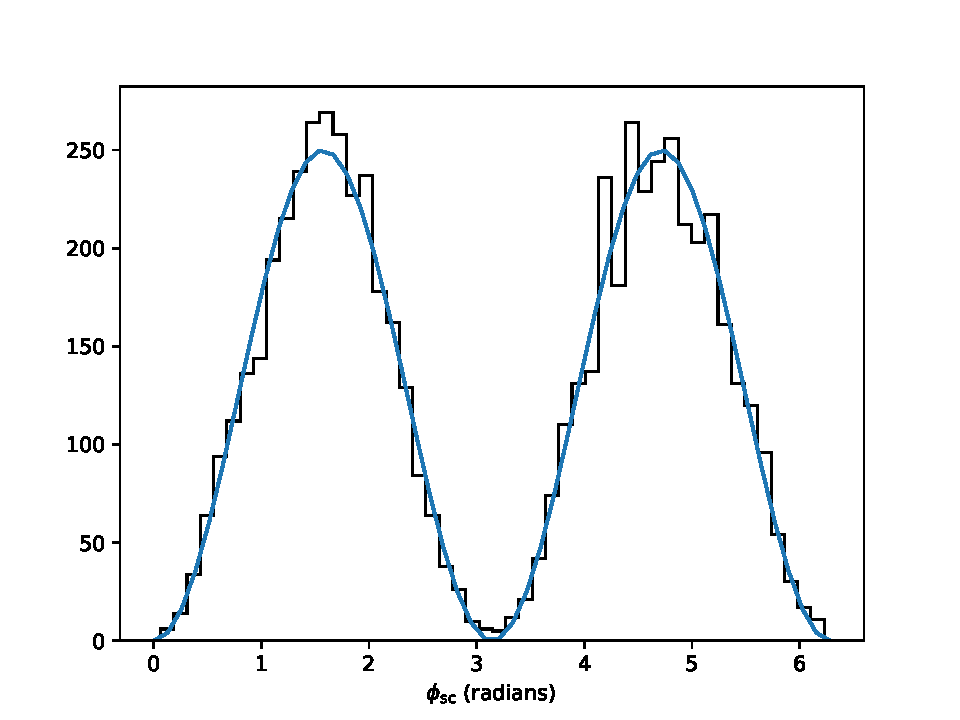
\includegraphics[]{phi_sampling_depaola}
 \caption{Plot of the distributed $\phi_\mathrm{sc}$ from sampling the Klein Nishina cross section as is outlined in Section \ref{mcrat} compared to the analytic cross section acquired by \cite{depaola2003new}. The distribution is shown in black and the analytic profile is shown by the blue curve.}
 \label{depaola_comparison}
 \end{figure}

\begin{figure}[]
 \centering
 \subfloat{
 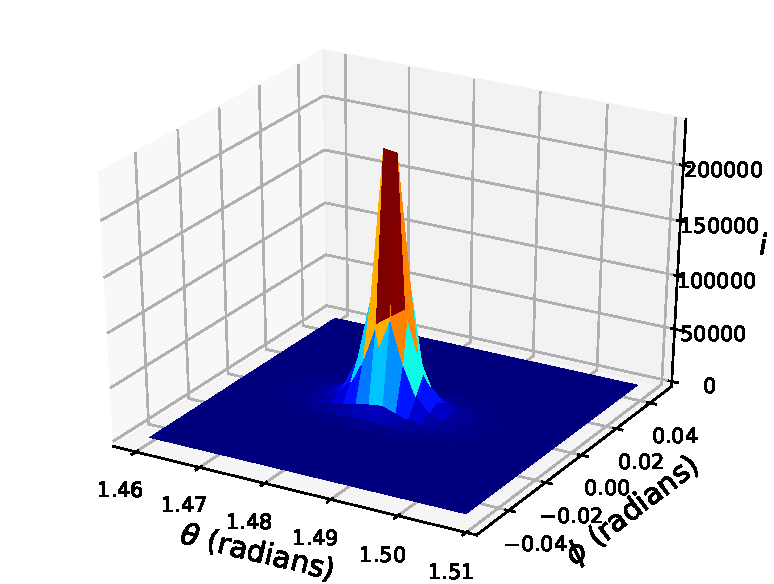
\includegraphics[width=0.5\textwidth]{kraw_test_i} %{0.5\textwidth} %{\label{kraw_i}}
 }
 \subfloat{
 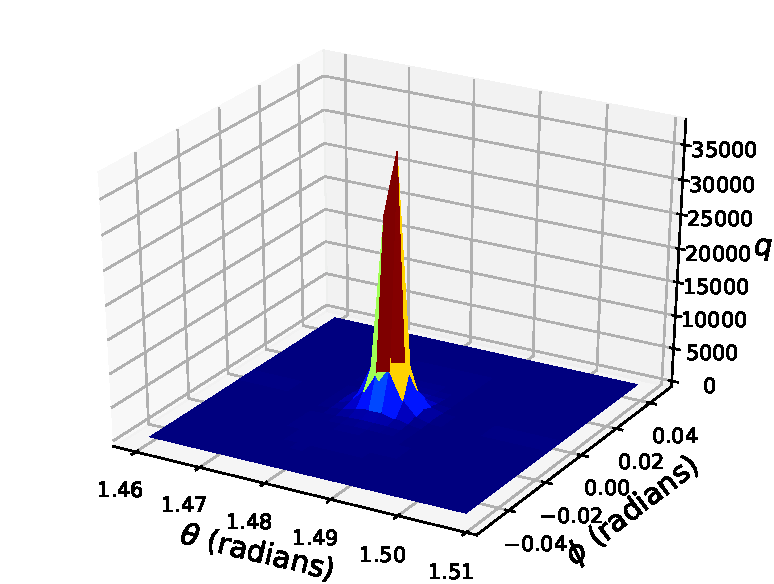
\includegraphics[width=0.5\textwidth]{kraw_test_q} %{0.5\textwidth} %{\label{kraw_q}}
 } \\
 \subfloat{
  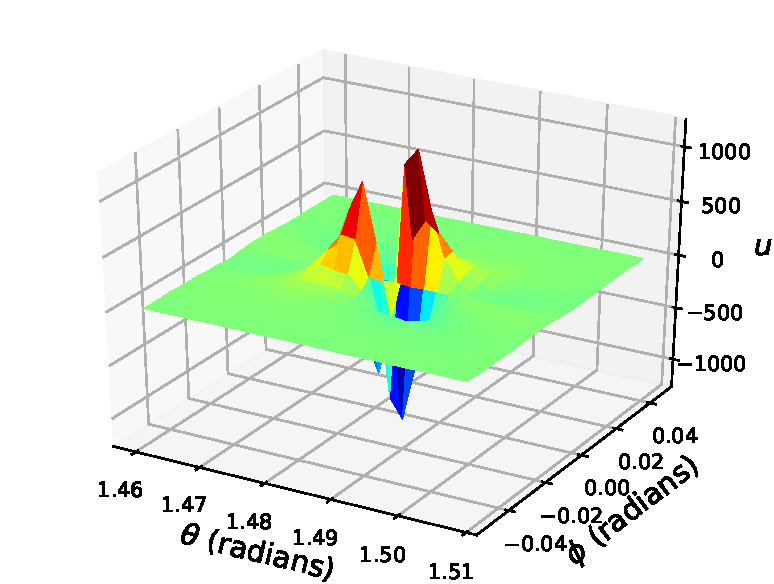
\includegraphics[width=0.5\textwidth]{kraw_test_u} %{0.5\textwidth} %{\label{kraw_u}}
  }
 \caption{The distribution of the stokes parameters as a function of the scattered photon's $\theta$ and $\phi$ values. These distributions are morphologically similar to the distribution acquired by \cite{krawczynski2011polarization} in thier Figure 6.  }
 \label{kraw_comparison}
 \end{figure}

In order to test the code globally, we reproduce the results of \cite{lundman2014polarization}. To do so, we imposed the analytic jet structure provided by \cite{lundman2014polarization} on the same simulation frames that we will use in Section \ref{results}. This is similar to \cite{MCRaT} simulating a variety of outflows by imposing an analytic solution onto hydrodynamic simulation files. {The domain of this simulation is $2.5 \times 10^{13}$ cm along the direction of the jet and $5 \times 10^{12}$ cm along the x axis.} We used $\sim 6 \times 10^5$ photons to conduct our code validation for a wide structured jet with $\theta_{\mathrm{j}}=0.1$ radians ($\sim 5.7^\circ$), $\Gamma_0=100$ and $L=3 \times 10^{50}$ erg/s. This is the same case exhibited in \citeauthor{lundman2014polarization}'s (\citeyear{lundman2014polarization}) wide jet with the exception of the value of $L$ that we use, which was chosen to maximize the number of photons that reached the photosphere before they approached the edge of the domain of the hydrodynamic simulation. {There are two major differences between the simulation conducted by \cite{lundman2014polarization} and the MCRaT simulation: 1) MCRaT uses the full Klein Nishina Cross section to determine if photons scatter while \citeauthor{lundman2014polarization}'s (\citeyear{lundman2014polarization}) simulation  uses the Thomson cross section and 2) The photons in MCRaT are not permitted to immediately escape to infinity if the randomly drawn optical depth is small enough while photons in  \citeauthor{lundman2014polarization}'s (\citeyear{lundman2014polarization}) simulation are allowed to do so. }

\begin{figure}
\centering
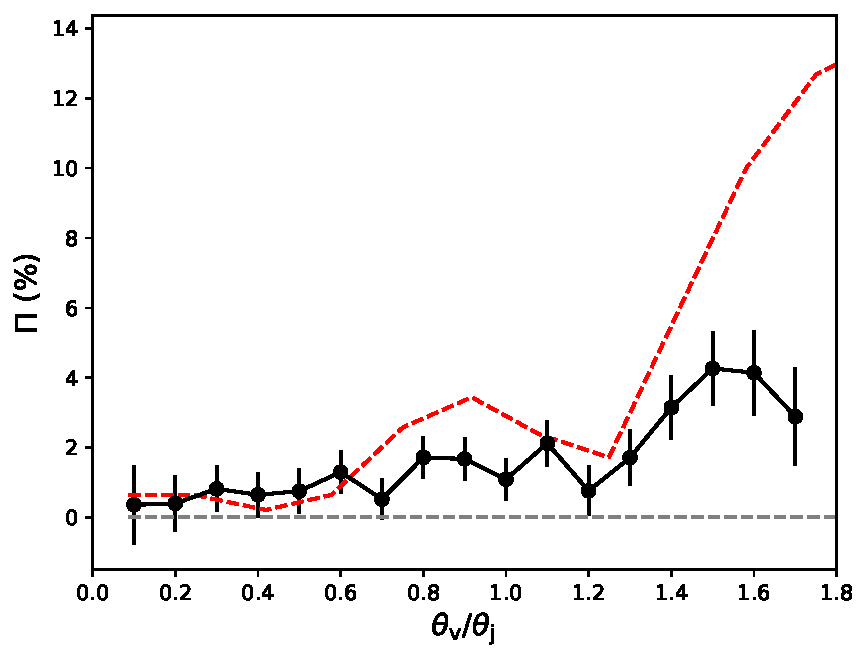
\includegraphics[width=\linewidth]{comp_lundman_p_4_thetaj_1e-01.pdf}
\caption{A comparison between the polarization acquired by \cite{lundman2014polarization} for a structured jet with $\theta_{\mathrm{j}}=0.1$ radians $\Gamma_0=100$ and $L=3 \times 10^{50}$ erg/s, shown by the {red} dashed line, and the MCRaT acquired polarization shown by the black points with $1\sigma$ error bars. The dashed grey line denotes $\Pi=0\%$ for reference. We find agreement until  $\theta_{\mathrm{v}}/\theta_{\mathrm{j}} \approx 1.6$ ($\theta_{\mathrm{v}} \approx 9^\circ$) where the MCRaT photons are no longer decoupled from the flow by the time they reach the edge of the simulation domain. }
\label{fig:complundmanp4thetaj1}
\end{figure}

In Figure \ref{fig:complundmanp4thetaj1} we show the results of our validation. The polarization acquired by \cite{lundman2014polarization} is shown as the red dotted line, the black points with $1\sigma$ error bars show the polarization acquired by MCRaT, and the grey dotted line shows $\Pi=0\%$ for reference. In addition to finding that the Stokes $u$ parameter vanishes ($\sum u \approx 0$), which is expected for an axis symmetric jet \citep{ito_polarization, lundman2014polarization}, we find that MCRaT is able to recover \citeauthor{lundman2014polarization}'s (\citeyear{lundman2014polarization}) polarization profile relatively well. {We are also able to recover the change in the sign of the stokes Q parameter at $\theta_{\mathrm{v}}/\theta_{\mathrm{j}} \sim 1.2$ that \cite{lundman2014polarization} find in their results.
The MCRaT result is slightly lower than the polarization acquired by \cite{lundman2014polarization} due to the fact that the analytic jet profile is mapped onto a discretized grid; this has the effect of decreasing the gradients in the jet profile that would contribute to a larger polarization. 
Furthermore, \citeauthor{lundman2014polarization}'s (\citeyear{lundman2014polarization}) polarization profile contains a minimum of 200 photons in each angle bin, while the results of the MCRaT validation contain at least $\sim 10000$ photons in each angle bin, increasing the general precision of the MCRaT results. }

For $\theta_{\mathrm{v}}/\theta_{\mathrm{j}} \gtrsim 1.6$ ($\theta_{\mathrm{v}} \approx 9^\circ$) the MCRaT polarization begins to decrease again, coming into strain with what is expected. This is due to the fact that the simulation files that we impose the analytic jet equations onto have a finite domain. Even when the photons reach the edge of the domain ($2.5 \times 10^{13}$ cm) at $\theta_{\mathrm{v}} \gtrsim 9^\circ$, they haven't fully decoupled from the photosphere (which would be located at $r\sim 1\times 10^{14}$ cm \citep{lundman2014polarization}) thus decreasing the detected polarization. 

\bibliography{references}
\end{document}